Encuentra el valor de la incógnita en el triángulo de la Figura \ref{fig:angle_triangle_10}.

\begin{minipage}[t][5cm][b]{0.3\textwidth}
    \begin{figure}[H]
        \centering
        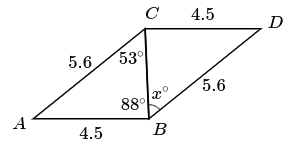
\includegraphics[width=0.99\linewidth]{../images/angle_triangle_10.png}
        \caption{}
        \label{fig:angle_triangle_10}
    \end{figure}
\end{minipage}\hfill
\begin{minipage}[t]{0.65\textwidth}
    \begin{solutionbox}{5cm}
        $\triangle ABC$ y $\triangle BCD$ tienen tres lados iguales. Comparten el lado
        $\overline{BC}$, las longitudes de $\overline{AB}$ y $\overline{CD}$ son iguales y las longitudes de
        $\overline{AC}$ y $\overline{BD}$ son iguales.
        \[\therefore \triangle ABC \cong \triangle BCD\]
        Los triángulos congruentes también tienen ángulos congruentes (iguales). Si superponemos estos dos triángulos, rotando
        $\triangle ABC$, observamos que el ángulo $x$ corresponde al
        $\angle ACB$ y $\angle ACB$ mide
        53$^\circ$.
        \[\therefore x=53^\circ\]
    \end{solutionbox}
\end{minipage}
